\documentclass[12pt]{article}

\usepackage{sbc-template}
\usepackage{graphicx,url}
\usepackage[utf8]{inputenc}
\usepackage[brazil]{babel}
\usepackage[utf8]{inputenc}  
\usepackage{xcolor}
\usepackage{multirow}
\usepackage{amsfonts}

\sloppy

\title{Árvores B e B\nolinebreak+ em Busca de Gravações de Música Clássica\\}

\author{Caio Stoduto\inst{1}, Lucas Guido\inst{1}, Nicolas Greco\inst{1},\\
Paulo Bezerra\inst{1}, Stephania Ferreira\inst{1}, Tales Bartolome\inst{1}}

\address{CMCC -- Universidade Federal do ABC (UFABC)\\
  Santo André -- SP -- Brazil
  \email{\{caio.stoduto,lucas.guido\}@aluno.ufabc.edu.br} \vspace{-1em}
  \email{\{nicolas.greco,paulo.bezerra\}@aluno.ufabc.edu.br} \vspace{-1em}
  \email{\{stephania.ferreira,m.bartolome\}@aluno.ufabc.edu.br} }

\begin{document} 

\maketitle

\begin{abstract}
  This meta-paper describes the style to be used in articles and short papers
  for SBC conferences. For papers in English, you should add just an abstract
  while for the papers in Portuguese, we also ask for an abstract in Portuguese
  (``resumo''). In both cases, abstracts should not have more than 10 lines and
  must be in the first page of the paper.
\end{abstract}
     
\begin{resumo} 
  Este meta-artigo descreve o estilo a ser usado na confecção de artigos e
  resumos de artigos para publicação nos anais das conferências organizadas pela
  SBC. É solicitada a escrita de resumo e abstract apenas para os artigos
  escritos em português. Artigos em inglês deverão apresentar apenas abstract.
  Nos dois casos, o autor deve tomar cuidado para que o resumo (e o abstract)
  não ultrapassem 10 linhas cada, sendo que ambos devem estar na primeira página
  do artigo.
\end{resumo}

\section{Introdução}
Dentro da música clássica, peças canônicas são gravadas centenas de vezes e,
para grande parte dos ouvintes, a escuta atenta de diferentes gravações é um
processo importante, permitindo a comparação das nuances de cada gravação~\cite{Bl:25}.
Assim, um sistema que permita a busca de gravações de uma música é essencial.
Os serviços de \emph{streaming} permitem acesso instantêneo e ilimitado a um
grande catálogo de músicas, facilitando o processo de escuta~\cite{MoVi:18}.
No entanto poucas plataformas de \emph{streaming} possuem funcionalidades focadas em
pesquisa de música clássica, tendo como foco maior a música popular~\cite{Bl:25}.
Assim sendo, a busca de música clássica nestes serviços é difícil e imprecisa, 
além de possuírem uma interface que não está alinhada a este estilo.
Por causa disso, as necessidades dos ouvintes de música clássica não são supridas
pelos grandes serviços de \emph{streaming}, como Spotify, Deezer e Youtube Music.

Tendo isso em vista, serviços dedicados à música clássica, tais como
IDAGIO, Apple Music Classical e Presto Music, foram criados e permitem busca
especializada, separando músicas de gravações, e interface considerando esta
divisão~\cite{Bl:25}.
Apesar de isto representar um avanço, a quantidade de plataformas ainda é pequena
e muitas delas ainda não estão bem estabelecidas, pois é um mercado nichado, e 
não há alternativas de código aberto, todas são iniciativas privadas e sem
detalhes acerca da implementação~\cite{Bl:25}.

Com base nisso, este trabalho objetiva implementar uma base de dados dedicada
para busca de peças de música clássica, de modo a permitir acesso mais
descentralizado a um sistema de busca, visando impulsionar o desenvolvimento de
novas soluções para este problema.
Para isso, serão utilizadas árvores B e B+ para a organização das informações,
pois estas são algumas das principais estruturas usadas no armazenamento de
informações em memória secundária~\cite{Co:79}.

O restante do artigo está organizado da seguinte forma:
a Seção~\ref{sec:revisao} apresenta informações sobre as árvores B e B+ e
trabalhos relacionados ao tema de pesquisa, a Seção~\ref{sec:problem} apresenta
em mais detalhes o problema de pesquisa. A Seção~\ref{sec:implementation}
descreve a implementação e as decisões tomadas para tal. A Seção~\ref{sec:results}
apresenta os resultados obtidos sobre a eficiência das implementações.
Por fim, a Seção~\ref{sec:conclusion} conclui o trabalho, com considerações
gerais e possibilidades de trabalhos futuros de modo a melhor explorar a temática.



\section{Revisão Bibliográfica} \label{sec:revisao}
Esta seção apresenta a fundamentação teórica das estruturas de dados utilizadas,
bem como outros trabalhos relacionados ao tema do presente artigo.

\subsection{Fundamentação Teórica}
Tendo em vista o uso de árvores B neste trabalho, esta seção tem como objetivo 
apresentar esta estrutura, sua utilidade e alguns resultados essenciais.

Durante o processo de manutenção de uma base de dados, um dos maiores custos
operacionais é o de acesso à memória secundária.
O acesso à memória secundária toma um tempo de ordens de magnitude maior do que
o tempo que o processador leva em instruções simples como de comparação de valores.
No entanto, diversas aplicações trabalham com uma quantidade de dados muito maior
do que a capacidade da memória principal financeiramente viável, o que torna o
acesso ao disco uma operação fundamental para o processamento de qualquer base
de dados e, ao pensarmos na otimização de tal processamento, a diminuição da
quantidade destes acessos ao disco pode se tornar o principal fator para o ganho
de performance operacional~\cite{clrs:22}.

Uma das soluções mais usadas para otimizar operações em memória secundária é o
uso de árvores B e suas variantes~\cite{Co:79}. Estas estruturas são árvores
nas quais cada nó pode armazenar mais que um registro, diferentemente das
árvores binárias.

Elas são definidas de modo que, considerando uma árvore não vazia de ordem
$d \in \mathbb{N}$, a raiz seja uma folha ou tenha no mínimo dois filhos, cada
nó diferente da raiz e das folhas possua entre $d+1$ e $2d +1$ filhos e todas as
folhas estejam no mesmo nível.
Além disso, pode-se concluir que cada nó que não é a raiz contém entre $d$ e $2d$
chaves e a altura $h$ da árvore está no intervalo
\[ \log_{2d+1} (n+1) \leq h \leq 1 + \log_{d+1} \left(\frac{n + 1}{2}\right)~\cite{SwMa:10}. \]

A característica de altura logarítmica se mostra muito importante, pois faz com
que operações de inserção e busca também tenham custo logarítimico.
Ademais, a possibilidade de armazenar diversas chaves em cada nó é adequada para
armazenamento em memória secundária pois possibilita tratar um nó como uma página % XXX o que é uma página?
em disco, de modo que a quantidade de leituras em memória secundária é minimizada~\cite{Kn:98}.

% Como apontado por Comer em seu artigo de 1979 \cite{Co:79}, a árvore B é uma
% estrutura de dados utilizada para a organização de um arquivo e os índices
% (também chamados chaves) de seus registros. Além disso, é uma generalização das
% árvores binárias balanceadas. No entanto, diferente das árvores binárias, cada
% nó de uma árvore B de ordem $t$ contém $n \in \mathbb{N}$ chaves, onde $t \le n
% \le 2t-1$, além de $n+1$ ponteiros por nó. Em consequência, o custo para
% as operações de busca, inserção e remoção crescem em proporção logarítmica com o
% aumento de registros do arquivo, o que representa um custo operacional
% relativamente baixo~\cite{Co:79}.

% Para acessar cada nó da árvore B, é necessário acessar a memória secundária.
% Apesar disso, seguindo as regras que definem a estrutura da árvore e seu
% balanceamento, em cada acesso é recuperado da memória não um registro, mas uma
% página de registros, de modo a se atingir uma pequena quantidade de acessos ao
% disco e a otimização dos processos de manipulação de registros do arquivo.

Já a árvore B+ é uma variação da árvore B, possuindo como
diferencial a ausência de registros em nós não-folha da estrutura, ou seja,
os registros estão contidos apenas nas folhas e as chaves estarão nos nós internos,
tendo um papel de guia na busca efetuada na árvore.
Além disso, os nós folha da árvore são ligados, de modo que é possível percorrer
os registros armazenados na árvore sequencialmente~\cite{Pm:10}.


\subsection{Trabalhos Relacionados}
Esta seção apresenta trabalhos relacionados a métodos de busca e indexação de 
músicas.

A indexação de pesquisas é um problema amplamente discutido em artigos ao longo
das décadas por conta de suas aplicabilidades no uso dos computadores,
principalmente com a emersão dos serviços de busca e \emph{streaming}.

O artigo de Nanopoulos et al. de 2009 discute o crescente campo de pesquisa dos
mecanismos de busca de música (\emph{Music Search Engines}), motivado pelo
crecimento exponencial da quantidade de músicas disponíveis na internet.
Os autores descrevem alguns dos critérios comuns para busca de músicas, que são
aplicados ainda atualmente em serviços de \emph{streaming}.
Alguns dos métodos incluem a busca através metadados relacionados a músicas (biografia de
artista, novos lançamentos, análises, entre outros), através de letra de música
e, para aumentar o leque musical de um ouvinte, há a recomendação de músicas
similares a escutadas e geração de playlists automáticas.
As duas formas apontadas de busca são por texto - por meio dos metadados, ou “smart words”,
que associam músicas a certas ocasiões (``músicas para ouvir no carro'' ou ``músicas
alegres'') - ou por conteúdo, incluindo características da música obtidas pelo áudio.

Na atualidade, os serviços de \emph{streaming} de música, como indicam Li et al. no seu
artigo de 2019 \cite{LiThChToGa:19}, precisam balancear mecanismos de busca específicos
e abrangentes a depender do usuário em questão.
Neste artigo, é feita a divisão em dois grupos: usuários focados e não focados.
O usuário com a mente focada, ao efetuar uma busca, procura algo em particular,
enquanto o não focado possui uma ideia vaga do que busca, estando aberto a
sugestões e efetuando pesquisas com frases mais subjetidas, reforçando alguns
dos métodos apresentados por Nanopoulos et al.

O método de busca utilizado neste trabalho visa um usuário focado, que já tem
conhecimento sobre que música deseja escutar e busca gravações específicas.
Assim, buscamos aperfeiçoar o conceito de busca focada, que, no contexto de Li et al.,
foi apresentado visando músicas em geral, para a música clássica.

Outro artigo que propõe uma alternativa para os métodos de pesquisa
usuais é o de Malhotra et al. (2022), com o algoritmo \emph{Pied Piper},
que apresenta um mecanismo de meta-busca de música \emph{pop} baseando-se em
três fatores: letras, metadados (como nome da música, artista, álbum, ano de
lançamento, andamento da música, tom, etc) e áudio (trechos ou gravações).
Com isso, foi proposta uma nova perspectiva que possibilitasse extrapolar as
limitações existentes em mecanismos clássicos de busca. Um dos diferenciais do
modelo seria a integração da busca de áudio, baseada no método conhecido como
\emph{Sequence-to-sequence Autoencoder Model for Audio Fingerprinting} (SAMAF)
\cite{Ba+:20}, que cria uma "digital" única para cada música, utilizada
em aplicativos como Shazam para identificar a música utilizando apenas trechos
curtos.
O método descrito aqui difere destes por ser exclusivamente baseado em metadados
textuais.

\section{Problema de Pesquisa} \label{sec:problem}

Levando em consideração o contexto de músicas clássicas, uma composição, feita
por um único compositor, possui diversas interpretações por diferentes músicos.
Com isso, uma necessidade relevante para os ouvintes desse estilo de música é a
busca dessas diferentes interpretações de uma composição de forma prática e
amigável, elevando a experiência do usuário.

Mesmo com isso em mente, poucas plataformas de \emph{streaming} de música levam
isso em consideração, pois se trata de um nicho dentro da imensa diversidade de
usuários, estilos e gêneros musicais.
Como exemplo, o comportamento do Spotify, uma das principais plataformas de
\emph{streaming} de música, não é adequado, pois, ao realizar uma pesquisa com o
nome da composição desejada, são exibidos resultados irrelevantes, como outras
músicas com nomes parecidos (tanto do mesmo compositor, como de outros), 
dificultando a busca por gravações da peça desejada.
A Figura~\ref{fig:spotify}, na qual foi feita a pesquisa ``Bach Trio Sonata no. 3'',
é um exemplo disso, pois nenhum dos resultados principais condiz com a música
pesquisada.

\begin{figure}[ht]
\centering
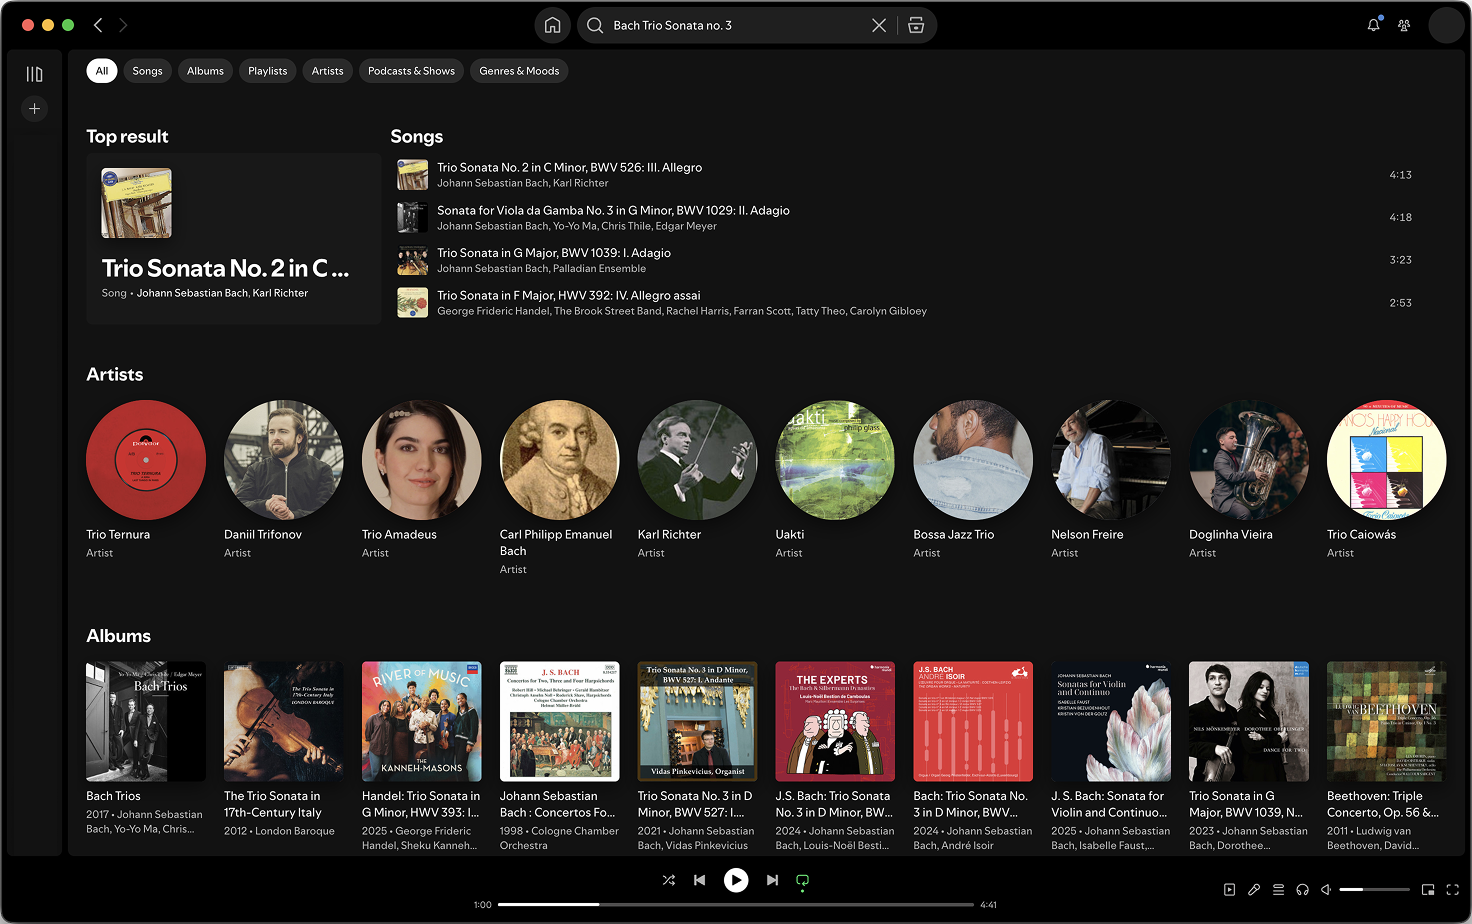
\includegraphics[width=1\textwidth]{figuras/Spotify.png}
\caption{Resultado de busca na plataforma Spotify}
\label{fig:spotify}
\end{figure}

Em contrapartida, existem plataformas de \emph{streaming} especializadas em
música clássica, como a plataforma IDAGIO e Presto Music, que adaptam seu
algoritmo de pesquisa especificamente para este nicho. Apesar disso, por se
tratar de um nicho limitado, há a grande iminência de um monopólio, por
existirem um número baixo de plataformas com funcionalidades voltadas para
ouvintes de música clássica. O principal exemplo desse movimento foi a aquisição
da antiga Primephonic pela Apple, criando a Apple Music Classical.
Com isso, surge a preocupação da estabilidade de um serviço de \emph{streaming}
nichado, como é o caso das plataformas dedicadas para música clássica, nas mãos
de uma empresa privada, que pode encerrar as atividades do serviço em caso de
diminuição da quantidade de ouvintes, posto que isso prejudicaria o lucro~\cite{Bl:25}.

Dado o exposto, este artigo cria uma implementação na seção seguinte de uma aplicação
computacional com o intuito de expandir o acesso a algoritmos especializados para busca
de músicas clássicas, respeitando a necessidade explicitada anteriormente, por
meio de uma prova de conceito. Isso implica a liberdade de qualquer usuário
poder usar a solução de código livre disponibilizada podendo adaptar às próprias
necessidades, como o uso em plataformas de \emph{streaming} ou em arquivos
locais. Além disso, possibilita a adoção desse sistema ou guia para criação de um sistema
próprio por empresas já estabelecidas neste mercado
para uma disponibilidade de funcionalidades mais
ampla dentre as plataformas, que resulta em refinamento nos seus mecanismos de busca e redução
da concentração destes sistemas em poucos serviços.

\section{Implementação} \label{sec:implementation}
Esta seção descreve as decisões de projeto tomadas para implementar as árvores
na resolução de nosso problema de pesquisa.

A implementação baseia-se na ideia de uma árvore de busca para o indexamento de
músicas clássicas, permitindo a obtenção de todas as gravações pelo termo de
busca, ou seja, informações sobre a composição. Para o desenvolvimento do sistema, foram
utilizadas duas alternativas de estruturas de dados semelhantes, as árvores B e
B\nolinebreak+ persistentes, permitindo que crie-se uma comparação direta entre
a eficiência em termos de complexidade de tempo, espaço e facilidade de
implementação.

Considerando a implementação, a estrutura de dados dentro das árvores B e
B\nolinebreak+ são usadas para guardar valores e registros. Com isso, o registro
guarda as seguintes informações:
\begin{itemize}
  \item Compositor (ex.: Ludwig van Beethoven);
  \item Nome da composição (ex.: Sinfonia no. 9);
  \item Catálogo (ex.: op. 125);
\end{itemize}

Além dessa estrutura, os metadados da música também compõem a própria chave,
sendo esta composta pela concatenação do Compositor e do Catálogo (ex:
"Ludwig van Beethoven125"). Com isso, o principal valor de busca presente no
valor dos elementos da árvore é o nome da composição. Com isso, a árvore serve
como um indexamento de dados atrelados a um conjunto de gravações, cabendo o
acréscimo de informações de outros tipos de metadados, como duração média,
quantidade de gravações, etc.

Além disso, para cada música, é criado dinâmicamente um arquivo único contendo diferentes gravações 
desta composição. Esse arquivo é armazenado na memória secundária com o caminho
atrelado aos metadados armazenados na árvore. A decisão da sequencialidade do
arquivo digital justifica-se pelo objetivo final da listagem de todas as
gravações, simplificando a implementação do projeto.

Com a problemática em mente, foi decidida a implementação do programa utilizando
a linguagem C++, pois ela apresenta um conjunto de características
imprescindíveis para o projeto. A principal característica é sua alta
performance, provindo da sua natureza de compilação \emph{Ahead-of-Time} (AOT),
juntamente com a possibilidade de trabalhar mais próximo às memórias primária e
secundária.
O quesito de tempo de execução é essencial para o projeto, já que o propósito é
uma ferramenta eficiente de busca.
Outra característica da linguagem que facilita a implementação é sua vasta
quantidade de bibliotecas que incorporam partes essenciais do código elaborado neste artigo.

Para a elaboração da implementação, foram utilizadas duas bibliotecas: 
\begin{itemize}
  \item ``disk-b-plus-tree''\footnote{\url{https://github.com/ByJuanDiego/disk-b-plus-tree}},
    que implementa uma árvore B+ baseada em disco, e
  \item ``TagLib''\footnote{\url{https://taglib.org/}},
    que possibilita a leitura de metadados de arquivos de música.
\end{itemize}
O uso destas bibliotecas permitiu abstrair partes complexas da implementação,
focando mais na aplicação envisionada.

\section{Resultados} \label{sec:results}
A presente seção descreve os resultados teóricos acerca das operações nas duas
árvores trabalhadas, bem como os resultados dos experimentos computacionais
feitos sobre as duas estruturas.

Sobre os aspectos teóricos, ambas as árvores apresentam complexidades assintóticas
de pior caso iguais, pois as operações são similares~\cite{Co:79}.
Destaca-se as complexidades de busca e inserção $O(d \log_d n)$, um dos aspectos
mais importantes destas estruturas, pois também permitem flexibilidade da estrutura
em decorrência da inserção eficiente.
É importante ressaltar que, por mais que a comparação de chaves textuais dependa
de seus tamanhos, nossas chaves possuem limite de tamanho, contribuindo, no pior
caso, apenas com um fator constante.

A eficiência das árvores B é ressaltada quando se tratando do caso de armazenamento
em memória secundária porque o maior custo está em recuperar as informações, e 
não nas operações em memória primária.
Assim, a principal medida de complexidade se torna a quantidade de leituras
realizadas, que é $O(\log_d n)$ em ambas as estruturas.

Apesar da similaridade das complexidades, a estrutura da árvore B+ é mais complexa,
armazenando uma lista encadeada com os registros e usando a árvore como índice
para os registros.
Por causa disso, o consumo de memória dela é maior que o da árvore B.
Além do mais, as buscas devem percorrer a árvore até as folhas, onde se encontram
os registros, de modo que é esperado que as operações sejam mais lentas.

\begin{table}[ht]
\centering
\caption{Tabela de Complexidades das Árvores B e B\nolinebreak+}
\label{tab:complexidades}
\begin{tabular}{|c|c|c|}
\hline
  Estrutura & Operação & Complexidade \\ \hline
  \multirow{4}{*}{Árvore B} & Espaço   & $O(n)$ \\
  \cline{2-3} & Busca    & $O(d \log_d n)$ \\
  \cline{2-3} & Inserção & $O(d \log_d n)$ \\
  \cline{2-3} & Remoção  & $O(d \log_d n)$ \\
  \hline
  \multirow{4}{*}{Árvore B\nolinebreak+} & Espaço & $O(n)$ \\
  \cline{2-3} & Busca & $O(d \log_d n)$ \\
  \cline{2-3} & Inserção & $O(d \log_d n)$\\
  \cline{2-3} & Remoção & $O(d \log_d n)$\\
  \hline
\end{tabular}
\end{table}

Para os experimentos computacionais, foram executados \emph{benchmarks} de tempo
de execução com base nas operações de mais importância, inserção e busca, nas duas
estruturas de árvores para comparar objetivamente as estatísticas de cada uma.
Para isso, foi executada uma inserção pseudo-randômica usando uma \emph{seed}
pré-definida que selecionou, dentre uma lista extensa de compositores extraído da
Wikipédia\footnote{\url{https://en.wikipedia.org/wiki/List_of_composers_by_name}},
autores, e, com base numa distribuição binomial com 20 tentativas com probabilidade
de sucesso 20.3\%, a quantidade de composições por gravação, permitindo uma
simulação comparável com casos reais.

Usando essa metodologia, foram rodados diversos testes variando a quantidade de
álbuns de 11 a 50001 para as duas árvores, armazenando o valor mínimo, médio e
máximo para cada variação, observado pela Tabela~\ref{tab:resultados}.
Estes resultados também estão apresentados de forma mais direta nos Gráficos das
Figuras~\ref{fig:graph_insert} e~\ref{fig:graph_search},comparando diretamente o
tempo médio de inserção e busca de cada árvore.

\begin{table}[ht]
\centering
\caption{Tabela de tempo gasto (ms) em operações nas árvores B e B e memória ocupada (bytes)\nolinebreak+}
\label{tab:resultados}
\begin{tabular}{|c|c|c|c|c|c|c|}
\hline
  Estrutura & Álbuns & Memória & Operação & Mínimo & Médio & Máximo \\ \hline
  \multirow{11}{*}{Árvore B} & \multirow{2}{*}{11} & \multirow{2}{*}{20512} & Inserção & 15.0585 & 27.9099 & 47.8788 \\
                            & & & Busca    & 0.0969 & 0.167911 & 1.3125	 \\
                  \cline{2-7} &  \multirow{2}{*}{101} & \multirow{2}{*}{135200} & Inserção & 7.0789 & 26.7159 & 96.4244\\
                            & & & Busca    & 0.2041 & 0.283696 & 2.2549	 \\
                  \cline{2-7} &  \multirow{2}{*}{1001} & \multirow{2}{*}{684064} & Inserção & 5.1006 & 21.5568 & 745.005 \\
                            & & & Busca    & 0.1968 & 0.258417 & 7.2308	 \\
                  \cline{2-7} &  \multirow{2}{*}{10001} & \multirow{2}{*}{831520} & Inserção & 4.8288 & 18.5928 & 7220.02  \\
                            & & & Busca    & 0.1844 & 0.245400 & 3.0743	\\
                  \cline{2-7} &  \multirow{2}{*}{50001} & \multirow{2}{*}{856096} & Inserção & 4.8917 & 26.7119 & 41062.2\\
                            & & & Busca    & 0.2019 & 0.285582 & 5.2455	 \\
  \hline

  \multirow{11}{*}{Árvore B\nolinebreak+} & \multirow{2}{*}{11} & \multirow{2}{*}{12098} & Inserção & 8.0324 & 39.1596 & 48.9896\\
                            & & & Busca    & 1.5894 & 2.12140 & 79.6278	 \\
                  \cline{2-7} &  \multirow{2}{*}{101} & \multirow{2}{*}{95342} & Inserção & 9.2234 & 42.5022 & 178.4730 \\
                            & & & Busca    & 1.4827 & 1.95975 & 20.4496	 \\
                  \cline{2-7} &  \multirow{2}{*}{1001} & \multirow{2}{*}{845314} & Inserção & 8.2050 & 35.8312 & 780.460\\
                            & & & Busca    & 1.5804 & 1.82577 & 8.8614  \\
                  \cline{2-7} &  \multirow{2}{*}{10001} & \multirow{2}{*}{8527230} & Inserção & 7.7294 & 33.0609 & 7384.99 \\
                            & & & Busca    & 1.6700 & 1.95760 & 12.3330	 \\
                  \cline{2-7} &  \multirow{2}{*}{50001} & \multirow{2}{*}{53585465} & Inserção & 8.1941 & 37.5146 & 42112.9\\
                            & & & Busca    & 1.6981 & 2.09856 & 336.733	 \\
  \hline
\end{tabular}
\end{table}

\begin{figure}[ht]
\centering
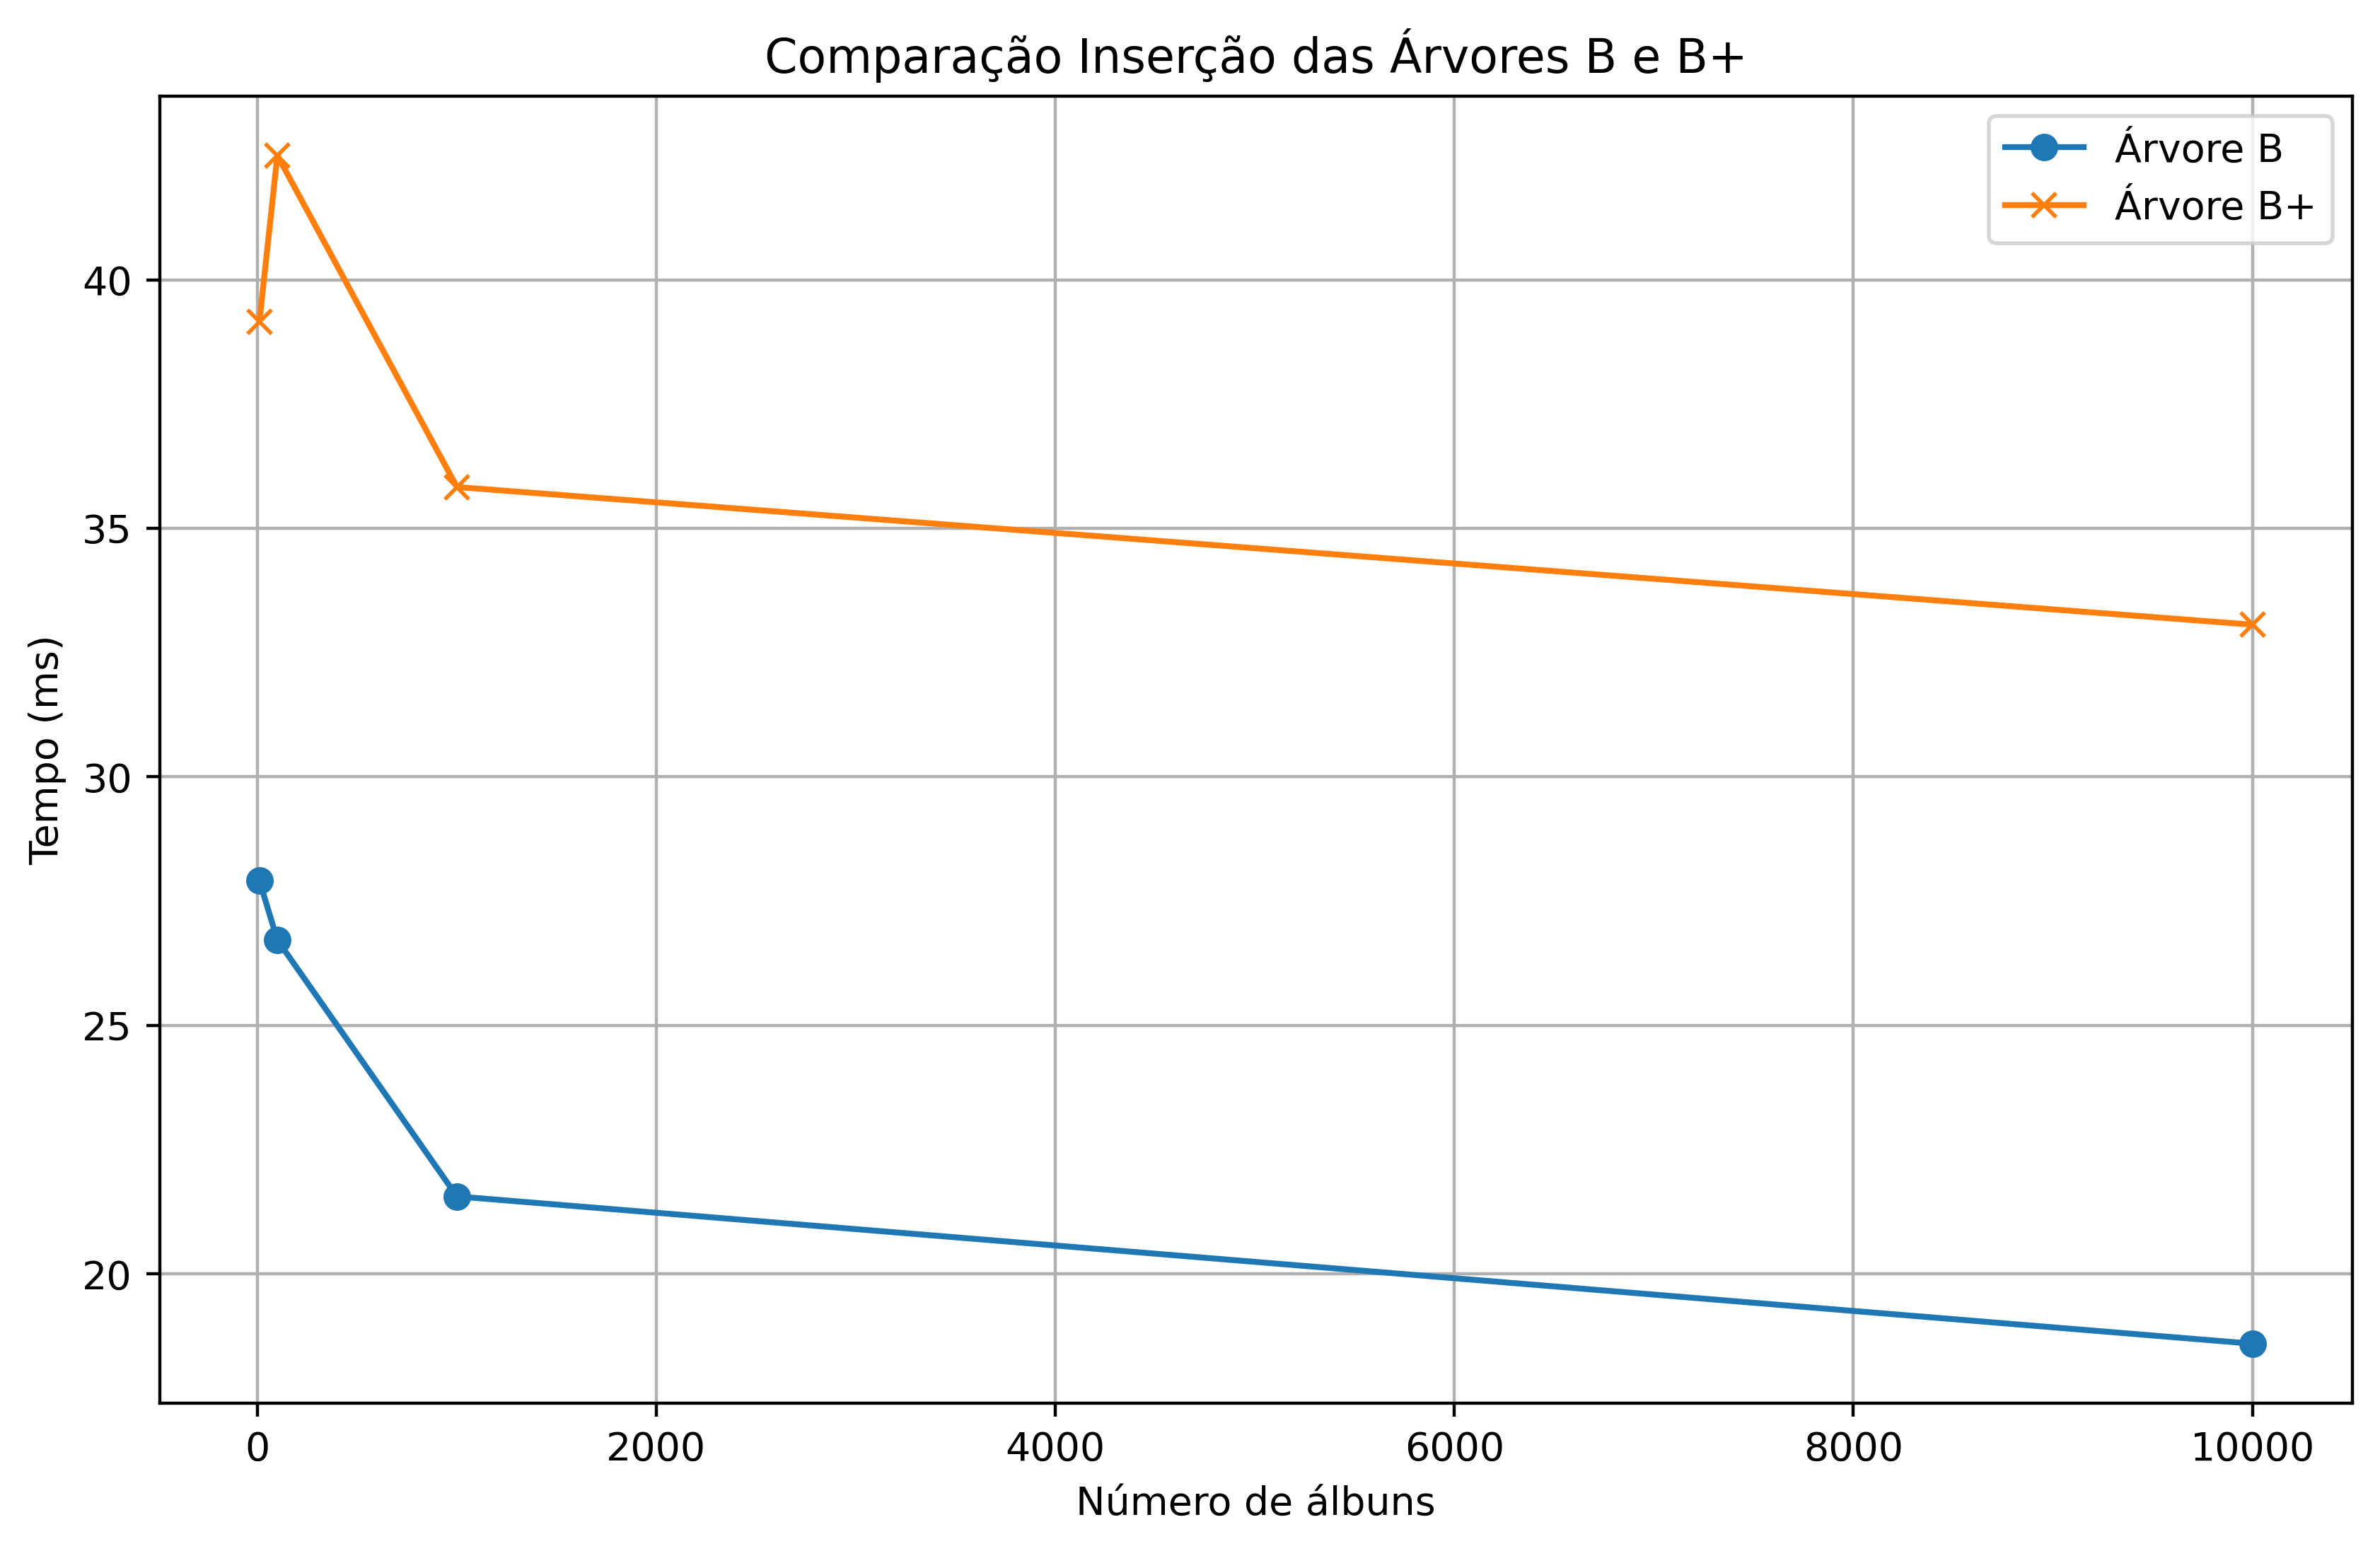
\includegraphics[width=1\textwidth]{figuras/graph_insert.png}
\caption{Resultado do tempo de execução da operação inserir}
\label{fig:graph_insert}
\end{figure}

\begin{figure}[ht]
\centering
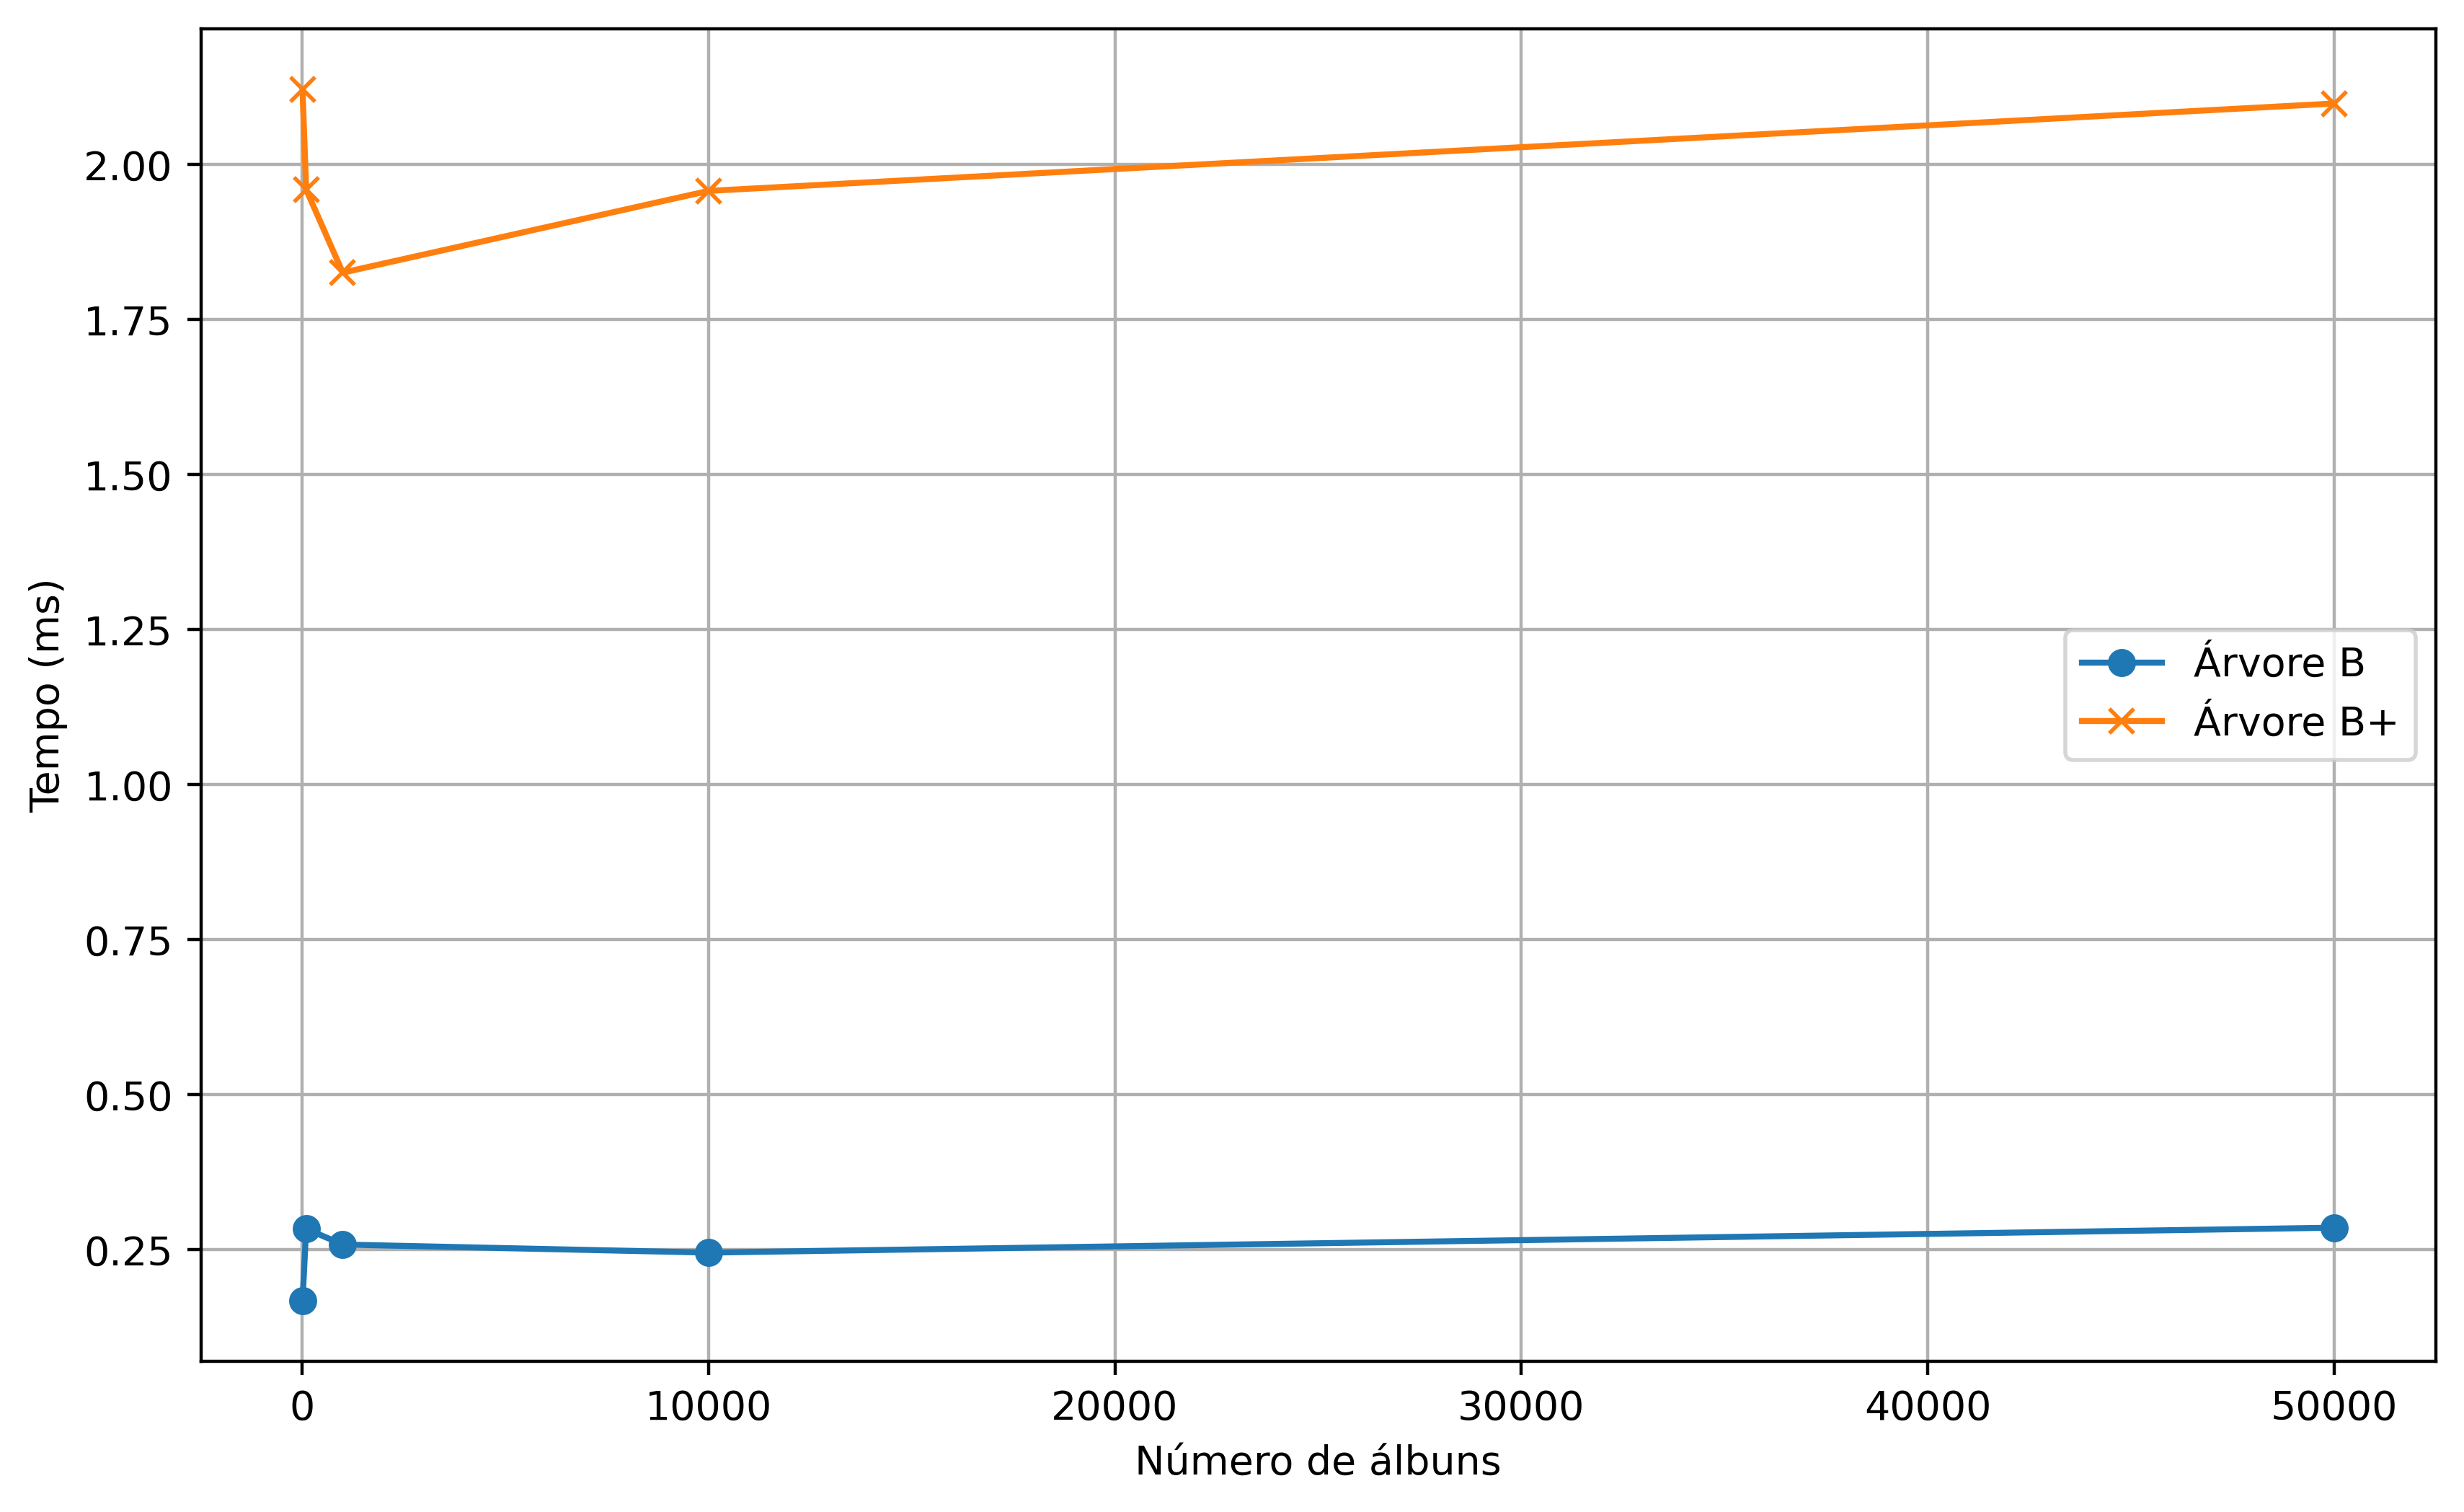
\includegraphics[width=1\textwidth]{figuras/graph_search.png}
\caption{Resultado do tempo de execução da operação buscar}
\label{fig:graph_search}
\end{figure}

A partir dos dados de \emph{benchmark}, é perceptível que as operações na árvore B
foram mais rápidas, com destaque para a operação de busca, que superou por uma 
grande margem a árvore B+.

Por fim, comparando os resultados teóricos com os práticos, a tendência logarítimica
esperada pôde ser observada.
Nota-se, no entanto, uma divergência no início dos gráficos, que pode ser explicada
pelas constantes dos algoritmos, desconsideradas pela análise assintótica, que
foca em analisar as tendências de crescimento.
Ademais, a expectativa de que a árvore B performaria melhor que a B+ foi corroborada
pelos experimentos computacionais, demonstrando que, para esta aplicação, a
melhor escolha é a estrutura de árvore B, posto que não são utilizadas as 
vantagens da árvore B+, como a possibilidade de percorrer os registros sequencialmente.

\section{Conclusão} \label{sec:conclusion}
Este artigo buscou explorar formas de preencher o nicho de busca por gravações
de música clássica, que permanece explorado por um número pequeno de empresas.
Para isso, foram utilizadas árvores B e B+ para indexar gravações com base na
composição.

Diante dos dados apresentados, pode-se concluir que ambas as árvores podem ser
utilizadas para esta aplicação.
A árvore B se mostrou satisfatória, no entanto, a árvore B+ se mostrou menos
eficiente, devido à sua maior complexidade.
Como o acesso sequencial de registros, possibilitado por esta estrutura, não foi
utilizado em nossa implementação, não se justifica o seu uso, tendo em vista o
maior tempo de busca, maior memória utilizada e maior complexidade de implementação.

Possibilidades de trabalhos futuros incluem o uso de diferentes estruturas para
a indexação, como a possibilidade de utilizar Hash para transformar o nome do
compositor em um valor numérico, ou estruturas dedicadas para busca de chaves
textuais, como as árvores digitais.
Ademais, um dos principais problemas desta abordagem é a necessidade de metadados
consistentes para todas as gravações armazenadas, de modo que seria possível
explorar formas de tratar os metadados de forma automática, por meio de
aprendizado de máquina, por exemplo.


\bibliographystyle{sbc}
\bibliography{bibliography}

\end{document}
